%%%%%%%%%%%%%%%%%%%%%%%%%%  phdsymp_sample2e.tex %%%%%%%%%%%%%%%%%%%%%%%%%%%%%%
%% changes for phdsymp.cls marked with !PN
%% except all occ. of phdsymp.sty changed phdsymp.cls
%%%%%%%%%%                                                       %%%%%%%%%%%%%
%%%%%%%%%%    More information: see the header of phdsymp.cls   %%%%%%%%%%%%%
%%%%%%%%%%                                                       %%%%%%%%%%%%%
%%%%%%%%%%%%%%%%%%%%%%%%%%%%%%%%%%%%%%%%%%%%%%%%%%%%%%%%%%%%%%%%%%%%%%%%%%%%%%%


%\documentclass[10pt]{phdsymp} %!PN
%\documentclass[twocolumn]{phdsymp} %!PN
%\documentclass[12pt,draft]{phdsymp} %!PN
%\documentstyle[twocolumn]{phdsymp}
%\documentstyle[12pt,twoside,draft]{phdsymp}
%\documentstyle[9pt,twocolumn,technote,twoside]{phdsymp}
\documentclass[a4paper,oneside,12pt]{article}

\usepackage{pdfpages}
\usepackage{a4wide}
\usepackage[english]{babel}
\usepackage{url}
\usepackage{caption}
\usepackage{multirow}
\usepackage{rotating}
\usepackage{soul}

\usepackage{palatino}

\usepackage{graphicx}
\graphicspath{{figures/}}
\def\BibTeX{{\rm B\kern-.05em{\sc i\kern-.025em b}\kern-.08em
    T\kern-.1667em\lower.7ex\hbox{E}\kern-.125emX}}

\newtheorem{theorem}{Theorem}

% zet de paragrafen een beetje uit elkaar en links uitgelijnd
\setlength{\parindent}{0mm}
\setlength{\parskip}{1ex plus 0.5ex minus 0.2ex}

\setlength{\textheight}{23cm}
\setlength{\textwidth}{16cm}
\setlength{\oddsidemargin}{0cm}
\setlength{\evensidemargin}{0cm}
\setlength{\topmargin}{-1cm}

\penalty-10000
\tolerance=10000

% \setlength{\parskip}{0pt}
% \setlength{\parsep}{0pt}
% \setlength{\headsep}{0pt}
% \setlength{\topskip}{0pt}
% \setlength{\topmargin}{0pt}
% \setlength{\topsep}{0pt}
% \setlength{\partopsep}{0pt}

\linespread{0.9725}

\usepackage[compact]{titlesec}
%\titlespacing{\section}{1pt}{*0}{*0}
%\titlespacing{\subsection}{1pt}{*0}{*0}
\titlespacing{\subsubsection}{1pt}{*0}{*0}

\usepackage{mdwlist}

\begin{document}


%-------------------------------------------------------------------------------------------

\thispagestyle{empty}

\begin{center}
\mbox{}\\\vspace{5mm}
{\large Research Proposal Accompanying Application for CSC Grant}\\ [45mm]
%
{\bf\Large Hardware Acceleration for FPGA CAD Tools by Efficiently Parallelizing PAR onto GPU/FPGA} \\
%[3mm] Concurrent Place and Route algorithms for Hardware Accelerators GPU/FPGA} \\
\vspace{45mm}
\large Applicant: Yun ZHOU \\
\vspace{2mm}
\small\texttt{zhouyun\_zy@foxmail.com} \\
\vspace{10mm}
\normalsize SouthWest Jiaotong University, China \\
\normalsize School of Information Science and Technology\\
\vspace{10mm}
\large Advisor: ir.\ Elias Vansteenkiste \\
\small\texttt{Elias.Vansteenkiste@ugent.be} \\
\vspace{2mm}
\large Promotor: prof.\ dr.\ ir.\ Dirk Stroobandt \\
\small\texttt{Dirk.Stroobandt@ugent.be} \\
\vspace{10mm}
\normalsize Ghent University, Belgium \\
\normalsize Department of Electronics and Information Systems\\
\normalsize Computer Systems Lab\\
\normalsize Hardware and Embedded Systems Group
\end{center}

\newpage

\tableofcontents

\vspace{5mm}
\begin{description*}

\item[Personal profiles]\ \\

\emph{Name of Applicant:} Yun ZHOU
\hspace{10mm}\emph{Gender:} Female
\hspace{10mm}\emph{Nationality:} Chinese\\
\emph{Date of Birth:} October 2, 1992
\hspace{13mm}\emph{Phone Number:} +86 18782186684\\
\emph{Degree:} Bachelor's Degree in Electronic and Information Engineering\\
\emph{Institution of Applicant:} School of Information Science and Technology, SouthWest Jiaotong University, China\\
\emph{Institution to Which the Applicant is Applying:}\\
Department of Electronics and Information Systems, Ghent University, Belgium
\end{description*}
\begin{description*}
\item[Signature of the Promotor:]\ \\
\item[Date:]\
\end{description*}
\clearpage

\section{Problem Definition}
A Field Programmable Gate Array (FPGA) is an integrated circuit made up of a grid of programmable functional blocks embedded in a programmable interconnection network. An FPGA can be reconfigured  at boot time by writing a different bitstream to the configuration memory, which makes it remarkably flexible to implement any arbitrary digital circuit.
Mainly due to their flexibility that leads to a substantial reduction of the economic risk of developing hardware accelerators, FPGAs are becoming ubiquitous components in digital systems and datacenters \cite{ovtcharov2015accelerating,putnam2015reconfigurable}. The flexibility also explains the rise in the popularity of the FPGA~\cite{putnam2015reconfigurable}.

Unfortunately the flexibility of the FPGA comes at a price. Designers typically needs to compile his application numerous times to test if his/her design meets the constraints of the application. Each time the design has to be compiled to an FPGA configuration and this is a complex and time consuming process, relying heavily on the FPGA computer-aided design (CAD) tools developed to compile a bitstream starting from a high level description.
However, the power of the FPGA CAD tools lags behind when FPGA devices and application sizes still keep increasing, following Moore's law~\cite{shannon2015technology}. The traditional CAD heuristics scale very badly in terms of application and device size, which translates to waiting times of hours up until days for compilation to be finished \cite{murray2015timing}.
Reducing the compilation time to improve the efficiency of CAD tools has become an active research field.

%The main FPGA device manufacturers and the academic community have developed a chain of heuristics to solve the NP hard problems involved in the compilation.
The compilation/translation of the FPGA CAD tool flow is typically divided into five steps: synthesis, technology mapping, placement, routing and configuration, dealt with by separate tools.  %An overview of the tool flow is given in Figure \ref{toolflow}. %In each step NP hard problems have to be solved and heuristics were and are being developed to try to approximate an optimal solution.
Runtimes of the different steps in the compilation of the toolflow can be indicated by the pie chart in Figure~\ref{rt}. These were obtained for the popular academic tool flow Verilog-To-Routing~\cite{luu2014vtr} and for the commercial tool flow from Xilinx, Vivado \cite{feist2012vivado}, using the framework in~\cite{vansteenkiste2015analyzing}. As also stated by other important publications, such as \cite{murray2015timing}, the most time-consuming steps are the placement and routing (PAR) steps, which have to be performed to obtain the needed accurate timing information to assess if the design meets the constraints.
Therefore reducing PAR time is of great importance to reduce the overall runtime of the CAD flow.
%They are the last steps at the backend of the tool flow.
%These steps have to be performed to obtain accurate timing information, which is needed to assess if the design meets the constraints.

%Additionally, FPGA devices and application sizes are still increasing, following Moore's law~\cite{shannon2015technology}. Unfortunately the power of the FPGA CAD tools lags behind. The traditional CAD heuristics scale very badly in terms of application and device size, which translates to waiting times of hours up until days for compilation to be finished \cite{murray2015timing}.

%Since the introduction of high-level synthesis~\cite{autoesl}, more and more engineers with a software background attempt to accelerate applications with an FPGA. They are used to gcc-like compilation times. Their design methodologies are adapted to these short compilation times. In order to fix bugs and measure performance, the compilation would be performed numerous times, causing the undesirable long compilation times that are common in FPGA design.

One of the most promising approaches to keep the runtime of PAR in FPGA CAD tool flows reasonable is to develop multi-threaded versions of the heuristic algorithms \cite{ludwin2011,gort2012,betz2013method,jain2014multi}, but unfortunately scalability issues still exist and large designs still need hours to be compiled. To further speed up compilation, a straightforward path is to use hardware acceleration, but unfortunately the current multi-threaded algorithms for placement and routing are hard to adapt for the wide scale parallelisation used in hardware accelerators such as Graphics Processing Units (GPUs) and FPGAs, which support massively parallel computing.

Summary: \emph{FPGA design compilation takes too much time to allow efficient design turnaround times. Hardware acceleration of the compilation process is needed but the current placement and routing algorithms (see section \ref{existingapproach} for details)are not very well suited for this.
%Dynamische FPGA-herconfiguratie biedt vele voordelen. Op dit moment kan enkel de functionaliteit, maar nog niet het interconnectienetwerk van de FPGA gespecialiseerd worden op een automatische manier. Dit leidt tot veel manueel werk op het architecturaal niveau en dus heel dure en niet-herbruikbare implementaties.
}

\section{Research Objectives and Paths}

\paragraph{Research Objectives}
\emph{In this Ph.D. research proposal, the overall high level goal is to significantly reduce the FPGA design compilation time by efficiently parallelizing placement and routing algorithms onto a GPU/FPGA, in order to bring benefit to the developemnt of FPGA CAD tools and the design of FPGA based system. }
%For the routing problem, we envisage that the existing routing algorithms will not allow a significant enough efficiency increase. Therefore, in the second phase, we will investigate new routing algorithms that are much more susceptible to parallelization and are much more efficiently accelerated by hardware than the current implementations.
%The overall high level goal is to reduce the FPGA design compilation time, but in this proposal we mainly want to focus on placement and routing, because they are the main runtime consumers \cite{vansteenkiste2015analyzing}. %Therefore we assume the mapped circuit and FPGA architecture description as given.

What we want to investigate in the project is how much placement and routing can be accelerated by writing a specific GPU-kernel based on a massively parallelizable placement algorithm, with regard to the existing single-thread ones or the improved parallel ones that are performed on CPUs.
%\hl{I think here we can change it like this, distinct from the research objectives}
\paragraph{Research Paths}
The first step is to have a modified version of the placement algorithm {\sc Liquid} that can be implemented on GPU by parallelizing and improving it. {\sc Liquid} is a placement algorithm that is being developed at Ghent University \cite{liquid}.
The second is to implement the adapted version of {\sc Liquid} with Compute Unified Device Architecture (CUDA) \cite{nickolls2008scalable} and demonstrate and measure its performance.

Next comes the development of new routing algorithms that are much more susceptible to parallelization and much more efficiently accelerated by hardware than the current implementations. %Current graph based algorithms such as the omnipresent Pathfinder algorithm~\cite{pathfinder} are not suited for wide-scale parallelism.
We will investigate the introduction of new routing algorithms that can be massively parallelized for being accelerated by a GPU implementation. Another option is to use an FPGA to accelerate the routing algorithm. In both cases, significantly novel routing techniques will have to be developed to enable a significant efficiency increase of the routing algorithm implementation.


%\hl{Restrictions of the GPU} Although we have its restrictions in mind like the programming model the limited access, I think it would be better to not include this, because we propose to use GPU to accelerate the PAR, before the verification of whether it is efficient, it maybe better to not show this.


%\newpage
\section{Existing Approaches}
\label{existingapproach}

\begin{figure}[t]
\centering
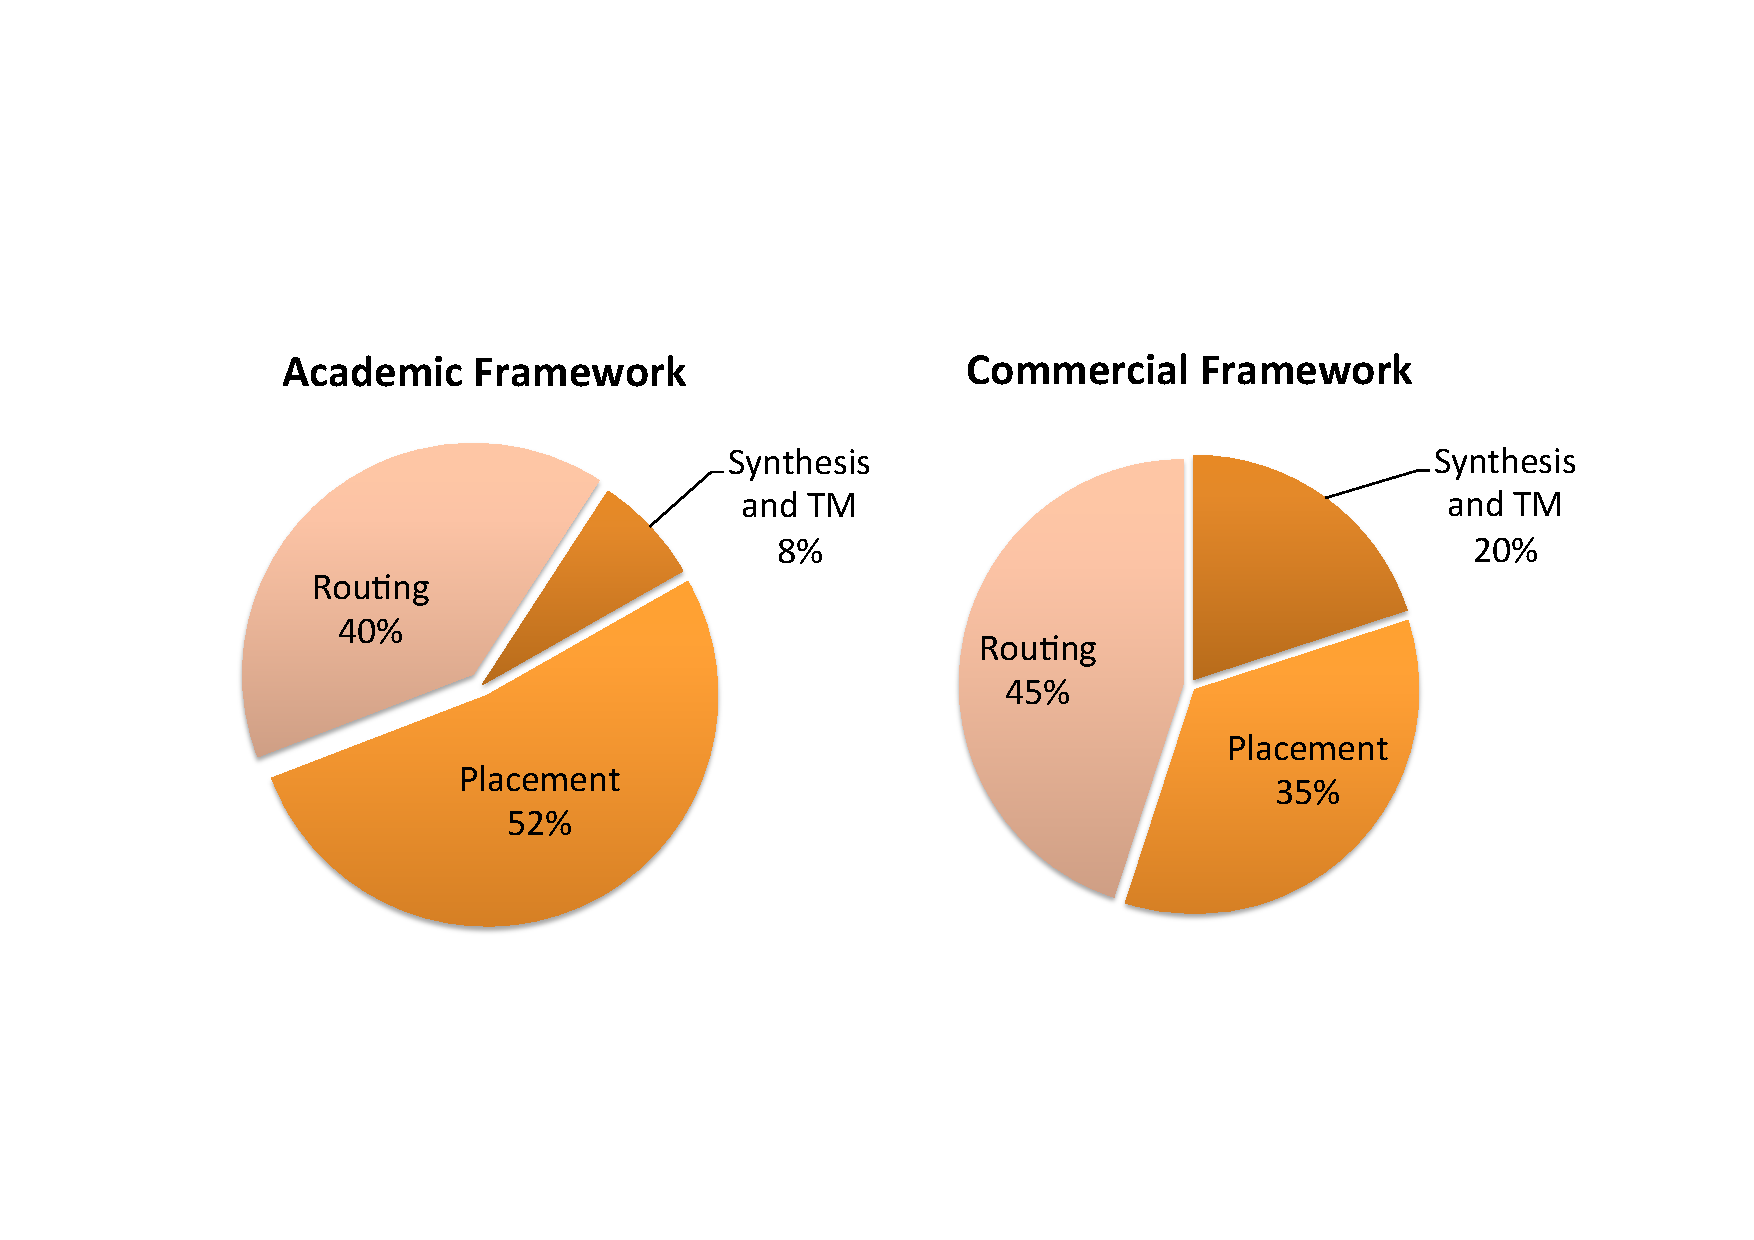
\includegraphics[width = 0.75\textwidth,trim = 0mm 50mm 0mm 40mm, clip]{runtime_breakdown}
\caption{Breakdown per tool of the compilation runtime.}
\label{rt}
\end{figure}



%\subsection{Existing approaches to Placement and Routing \hl{(1.5 pages)}}

\subsection{The FPGA Placement Problem}
\label{sec:placeprob}
%The problem
An FPGA placement algorithm takes two inputs: the mapped input circuit and a description of the target FPGA architecture. The algorithm searches a legal placement for the functional blocks of the input circuit so that circuit wiring is optimised. In a legal placement every functional block is associated to (placed on) one of the physical blocks (without overlap) that is capable of implementing the functional block.


%optimization goals
The main optimisation goal is to minimise the total wire length required to route the wires in the given placement. Placers that are only based on this goal are called wire-length-driven placers. More complex tools such as routability-driven \cite{swartz1998afrrff} and timing-driven placers \cite{marquardt2000tpff} trade some of the wire-length for a more balanced wiring density across the FPGA or a higher maximum clock frequency of the circuit, respectively.

%Dificult problem => Heuristic
%Easy to addapt => Simulated annealing
Finding a high quality placement is very important, because poor quality placements generally cannot be routed or lead to low operation frequencies and high power consumption. Worse, the placement problem is computationally hard, so there are no known algorithms that can find an optimal solution in a reasonable time. The two popular heuristical approaches are the simulating annealing based algorithm \cite{vprboek} and the analytical placement techniques \cite{chan2003ppffga}.

%\todo{Is dat eigenlijk wel waar dat SA placers gemakkelijkst aan te passen zijn? Heb je daar ook argumenten voor. Je kan wel zeggen dat deze p laatser met een kostfunctie werkt en enkel die kostfunctie aangepast moet worden maar de anderen zijn misschien even gemakkelijk aan te passen.}

\subsubsection{Simulated Annealing}
Simulated annealing \cite{kirkpatrick1983obsa} is inspired on annealing of metals, a technique involving heating and controlled cooling of a material to increase the size of its crystals and reduce their defects.
%\paragraph{The Basic Algorithm}%\hl{I think here you can significantly shorten.}
%At any time, the algorithm keeps track of the placement cost. In a wire-length-driven placer this is the sum of the estimated wire-lengths over all nets.
A detailed description of the algorithm can be found in \cite{kravitz1987placement}.
%The algorithm starts by randomly, but legally, placing the logic blocks in the input circuit on physical blocks of the FPGA architecture. Afterwards, the placer repeatedly tries to interchange the logic blocks placed on two randomly chosen physical blocks. Such an interchange is called a move. If the move causes a decrease in placement cost, the move is always accepted. If on the other hand, the move causes an increase in placement cost the move is accepted with a probability of $e^{-\frac{\Delta C}{T}}$, where $\Delta C$ is the change in cost due to the move and $T$ is a parameter called the temperature, which controls the probability by which hill-climbing moves are accepted. Initially, $T$ is very high so that most moves are accepted. Gradually $T$ is decreased so that the probability by which hill-climbing moves are accepted decreases. When the temperature is decreased in the proper way the result is a low cost placement. The hill-climbing moves allow the placer to escape from local minima.

The initial temperature, the rate at which the temperature is decreased, the number of moves that are attempted at each temperature, the way in which potential moves are selected and the exit criterion of the annealer are called the annealing schedule. A good annealing schedule is crucial for finding a good solution in a reasonable amount of time.

%\paragraph{Wire-length Estimation}
%\label{sec:wireLengthEstimation} The only way to exactly calculate the total wire-length of a given placement is to route the wires in a placement and sum the wire-length over all nets. Since routing is in itself a computationally hard problem, solving it repeatedly for every move tried in the inner loop of the placer and in this way exactly calculating the total wire-length, leads to very long execution times for the placer. Therefore, the cost is not exactly calculated but estimated.

%A common way of estimating is calculating the sum of the estimated wire lengths of each net, where the wire length of a net is estimated as the half-perimeter of its bounding box weighted by a factor which depends on the number of terminals of the net (taken from \cite{cheng1994raaeprm}). %It is equal to 1 for nets with up to three terminals and slowly grows to 2.79 for nets with 50 terminals.

\paragraph{Problems with using Simulated Annealing}
Typically the number of moves performed per temperature step is not linear with the number of blocks, which leads to long runtimes.
Although it seems straightforward to adapt simulated annealing for multiple threads, the quality of the solution and the speedup gain per thread deteriorate fast as the number of threads increase \cite{ludwin2011}. This is mainly caused by collisions and synchronization issues. In multi-threaded solutions each thread swaps blocks independently, instead of swapping blocks sequentially.

\subsubsection{Analytical Placement}
%In a analytical placement, the placement problem is represented as a linear system of equations.The optimal locations for the blocks in the circuit can be obtained by solving this linear system. The system of equations is obtained by taking the partial derivatives of the square of the total wire-length.Unfortunately the solution typically does not contain discrete block positions and blocks may overlap. However, placing blocks on the FPGA requires blocks to not overlap and the block positions are located at discrete positions.To overcome this, the solution is legalised resulting in a deteriorated placement.
In an analytical placement algorithm, the placement problem is represented as a linear system of equations that is built based on both the wire length of the connections and the distance to the legalized position, called anchor positions. These anchors are refreshed each time a solution is legalized.
Multiple iterations of solve-legalize are performed, while increasing the weight of the anchor connections. The algorithm typically stops if the decrease in cost of the legalized solution starts to slow down and converge towards the cost of the solved solution.  %The solution typically converges after 20 iterations, depending on how fast anchor weights are increased.

\paragraph{Problems with using Analytical Placement}
Each iteration the linear system is solved, it takes time to build it. A matrix of size NxN is to be constructed, with N being the number of connections. Although the matrix is sparse and can be stored efficiently with compressed row format, it requires extra memory, making analytical placement less scalable in terms of memory.
Both solving the linear system and the legalisation method are hard to parallelise and require synchronisation.

\subsection{The FPGA Routing Problem}
Once the placement algorithm has placed each of the logic blocks of the input circuit on a physical block of the FPGA architecture, the router needs to determine which of the switches in the routing architecture need to be closed and which need to be opened in order to connect the physical blocks in accordance to the way their associated logic blocks are connected in the input circuit. The goal is not only to find a legal routing solution but also to try to maximise the circuit clock frequency by allowing critical paths to use shorter and faster routing resources.

Most of the popular academic and commercial FPGA routers use a Pathfinder based algorithm\cite{vprboek,betz1997vanppartffr}.

\subsubsection{{\sc Pathfinder}: A Negotiated Congestion Router}
\label{sec:pathfinder}
\paragraph{Routing-resource Graph}
The routing-resource graph (RRG) is used as a model for the routing architecture of an FPGA in {\sc pathfinder} \cite{mcmurchie1995panprff}. It is a directed graph $C=(N,E)$, where the nodes $N$ represent the routing resources: wire segments, input pins, output pins, sinks and sources.

When the routing architecture of the FPGA is represented as a RRG, the routing algorithm will be reduced to finding a subgraph of the RRG, called a routing tree, for each of the nets. The algorithm stops when the routing trees of the nets are disjoint, which means no shared resources exist anymore \cite{nair1987asyetfgw}.
This is achieved by gradually increasing the cost of sharing resources between nets. During the first iteration, nets can share resources at no extra cost and thus, each net is routed with a minimum number of wires. The cost of a routing resource does not only depend on the current sharing cost but also on the sharing history of the resource. Resources that were shared heavily in past routing iterations become more expensive. In this way a congestion map is built, which enables nets to avoid routing through heavily congested resources, if possible.

\paragraph{Routing a Net}
The task of the net router is to find a minimum cost routing tree for a given net in the resource graph. The routing tree should contain the source and the sinks of the net and a path from the source to each of the sinks. The cost of the resources is determined by the negotiated congestion mechanism.

The search space of all possible routing trees for a net is huge. Therefore a heuristic was developed that finds a low cost routing tree for a given net in a reasonable amount of time. Typically a variant of a maze router is used~\cite{lee1961aafpcaia}. The maze router loops over all the sinks of the net and extends the already found routing tree with the shortest path from this routing tree to the sink under consideration. The shortest path is found using Dijkstra's algorithm \cite{dijkstra1959anotpicwg}.

Although the {\sc pathfinder} algorithm is very flexible because the RRG can be constructed for any useful routing architecture, it is not suited for wide-scale parallelism.

\begin{figure}[ht]
\centering
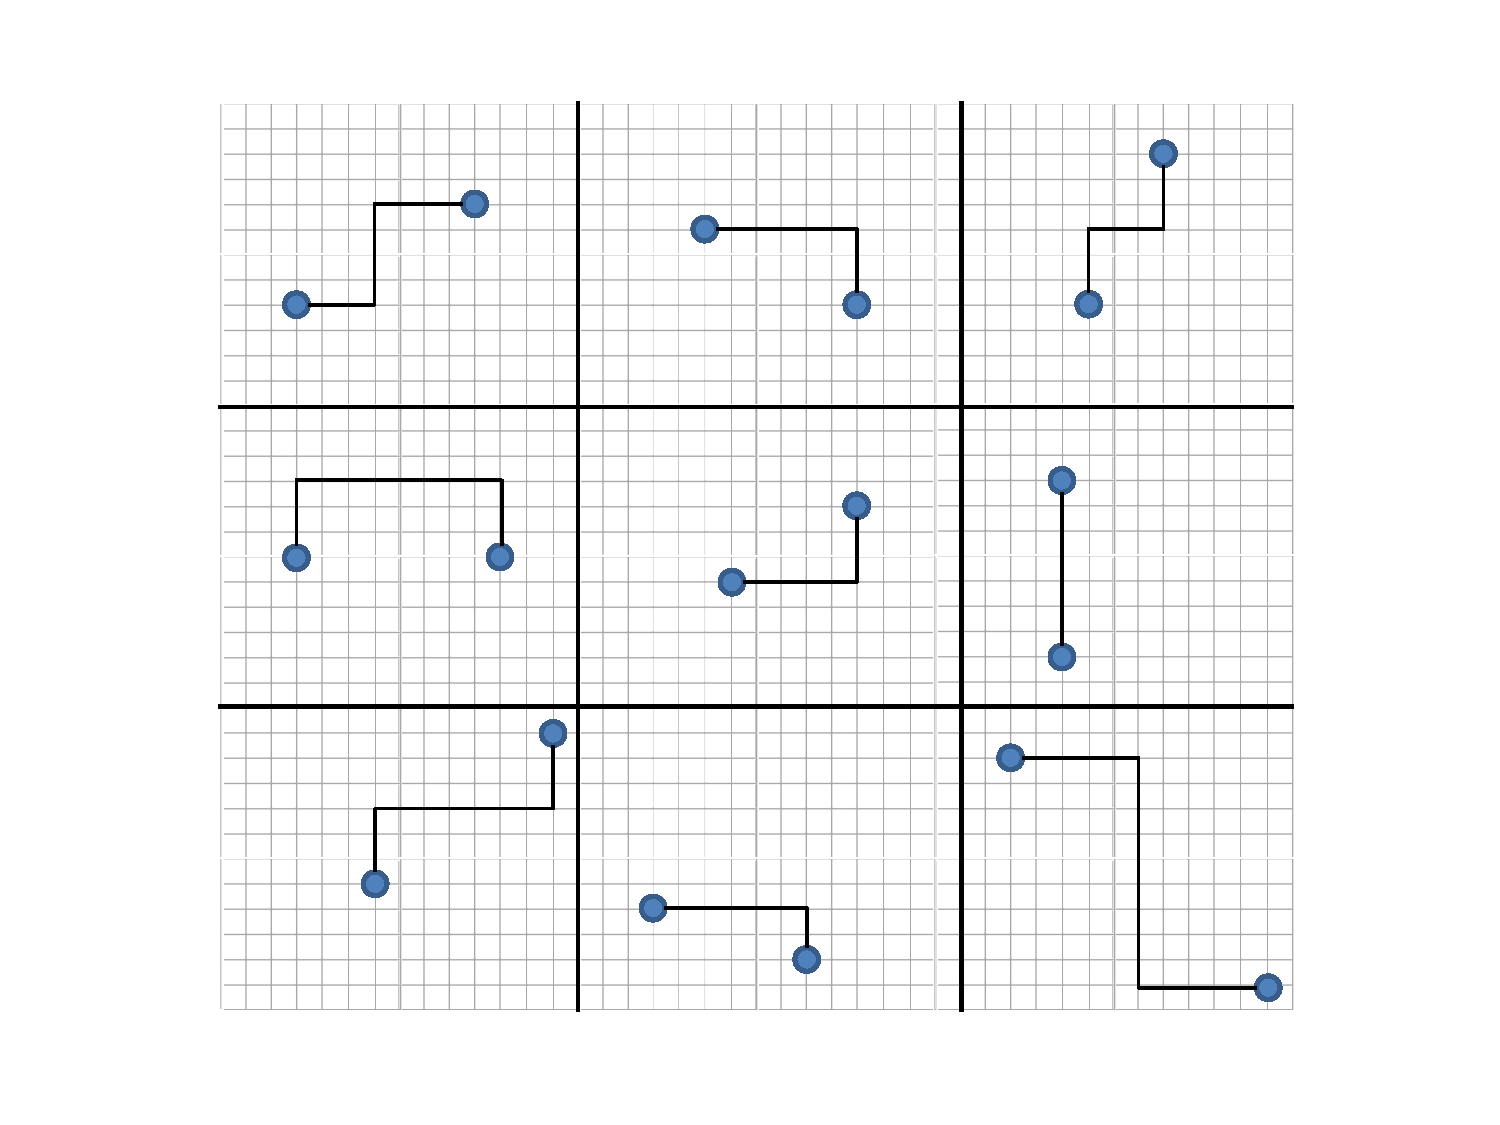
\includegraphics[width = 0.4\textwidth,trim = 0mm 0mm 0mm 0mm, clip]{parallellisatie}
\caption{Breaking up sets of nets based on the location of their terminals.}
\label{geopara}
\end{figure}

\subsubsection{State-of-the-art advances in routing techniques}
In~\cite{vansteenkiste2013connection} the authors were able to further refine the negotiated congestion mechanism to the level of connections. Nets are partially ripped up and rerouted, this allows us to only reroute congested connections, which helps us to avoid large routing runtimes for the large fanout nets. Others have developed multi-threaded routers. Gort et al. developed a multi-threaded router that splits up the nets in a circuit depending on the location of their terminals on the FPGA~\cite{gort2010deterministic}. Two nets can be routed concurrently in case they have terminals that are not located in each others bound box, as depicted in Figure~\ref{geopara}.
Another advance is the dynamic expansion of the routing resource graph, which leads to a reduction in memory usage~\cite{moctar2015fast}. 	
Adapting the routing architecture to speed up the routing is what the authors tried in~\cite{gort2013combined}.

%\newpage

\section{Proposed Techniques}


\subsection{Placement techniques}\label{placetech}

For placement we have a clear proposal, because the research group HES, that I would be part of, has developed a placement algorithm with large scale parallelism in mind. The algorithm is called {\sc Liquid} and a single threaded version is available~\cite{liquid}.

\paragraph{{\sc Liquid}}
{\sc Liquid} is based on analytical placement. It is also an iterative algorithm in which optimised placement and legalised versions of the placement are generated in each iteration. In contrast to analytical placement there is no linear system that is solved in each iteration. In each iteration all the blocks are moved a few times.  The blocks are moved in the direction of the steepest gradient descent. For each block a move vector is calculated based on the previous position of the other blocks that are attached to it. The cost function is the sum of the estimated routing and timing cost of the nets attached to the block. All movement vectors can be calculated independently, which makes it uniquely suitable for parallelisation.

%texture with all positions of previous locations

\paragraph{Legalizer}
In the current implementation the blocks are moved following the steepest gradient descent a few times before the positions are legalised. The legaliser tries to spread, the blocks and assign a legal position to each block without any overlapping blocks. Regions of overlapping blocks are gradually spread, but sometimes two regions clash while expanding the region. This and similar edge cases have to be captured and handled correctly. This is hard to make concurrent, because there are a lot of dependencies between the blocks.
Instead, our idea is to keep the movement of the blocks independent and introduce a legalising phase in which we will move the blocks a few steps not following the steepest gradient descent of the cost function, but trying to move each block to a legal position, while also repelling each other to prevent overlap. These moves will not lead to a completely legalised solution, but a nearly legalised solution. Based on experiments we know that it does not really influence the quality of the final solution if the intermediate solutions are not completely legalised.  At the end there will be one step of completely legalising, but this will be performed on the CPUs.

\paragraph{Timing analysis}
In a timing analysis the most critical connections are identified by traversing the timing graph. The connections determine the weights of the nets.
In the current implementation of {\sc Liquid}, we don't do a timing analysis after each optimize-legalise iteration, but we only do it each 5 iterations, because the criticality of the nets doesn't change extremely between iterations.
So there is an option to do timing analysis on the CPUs concurrently, while the moves are being performed by the GPUs, but it will be the subject of research if this will degrade the quality of result of the final placement.
Another research path will be to also adapt timing analysis to be able to run it on the GPU. This will involve accelerating breadth-first search, because that is one of the main components of timing analysis. This is not straightforward because it involves graph traversal and pointer chasing, but Merrill et al. showed significant speedups in \cite{Merrill2015}.



\subsection{Routing techniques}\label{routetech}

Many multithreading strategies for the routing problem have been proposed in the past, but the limitations of the SIMD architecture present in GPUs forces us to simplify the problem if we want to make use of the massive parallelism offered by the GPU.
In what follows we describe the different strategies that will be investigated during the Ph.D.\ research. Depending on the result, different strategies may be combined.

\paragraph{Route sets of connections in parallel}
As mentioned in Section~\ref{existingapproach}, the first routing iteration takes the largest portion of runtime because each connection needs to be routed.
It is important that the connections in the first iterations are routed independently because in the first iteration the router typically does not take into account congestion cost, but only delay.

Enlightened by the popularity of the A* path-finding search algorithm in large-scale games for concurrently finding the shortest distance between two nodes in a speedy way, we can perform multiple A*-search in the routing resource graph of the FPGA to route the connections in parallel. Making use of GPU's highly parallel multi-threaded nature suits this scenario perfectly \cite{bleiweiss2008gpu,bleiweiss2012system}.

All A*-search wavefronts will be started in parallel. Each thread will behave as a single router and will have its own priority queue. The instructions will be the same for all the router threads and can therefore be executed in one warp. Pop a node from the priority queue. Check if the target is reached and if not add the neighbours to the priority queue. After each router thread finds its target, a new warp can be started with threads that backtrace the path that lead to the target. Each thread spawns its own routing trace on a per cycle basis. For each connection there will be one backtrace thread. All backtrace threads will have the same instructions. They are also responsible for producing a series of history congestion cost updates. These updates are used after a batch of connections is done to build/update the congestion map.
% foreseeable problem: investigate visitation statuses of the nodes in the graph

\paragraph{Parallelize the Search}
A finer grained approach is parallelizing the A*-search in itself. The wavefront is expanded by different threads. A fixed number of nodes are popped from the priority queue and each thread processes the node separately. Each thread checks if the target is reached and if not the cost of the neighbouring nodes is calculated and added to the priority queue in a similar way as done in~\cite{Merrill2015}. The wavefront of an A*-search is typically directed towards the goal and so it only makes sense to expand a limited amount of nodes at a time, so we suggest to use the maximum number of threads in one warp, this is typically 32. This finer grained approach could be applied in the later router iterations in which the negotiated congestion mechanism is more sensitive to synchronization and connections have to be routed one after the other or only connections in other locations can be routed concurrently~\cite{gort2010deterministic}.

\paragraph{Tile based Compression of the Routing Resource Graph}
The routing resource graph (RRG) is actually built up of stitched instances of a few regular tiles. An expanded RRG can easily surpass today's workstation memory capacities \cite{murray2015timing}. It is important the routing resource graph fits in the GPU memory banks.
An FPGA consists of a grid of logic blocks interspersed with columns of memory blocks and DSP blocks. The interconnection fabric surrounding each type of block is typically adapted to the size and the number of I/O of the block. For each tile type a template RRG tile can be kept in the shared memory of the router threads. It is constant and read-only.
Tile-based compression of the RRG has been attempted in the past \cite{chin2007memory}, but was only evaluated in a single thread implementation on a CPU.

%Elias -> Dirk: In case you have any ideas about this let me know or you could write something up by yourself.
%\paragraph{Move away from graph based routers}
% Routing resource graph
%graph based
%move away from graph based routing algorithms

%\subsection{GPU Programming with CUDA}



\section{Experimental Evaluation and Expected Outcomes}

All experiments will be conducted on a host machine with a dual socket, dual core 2.27 GHz processor and 4 GB of memory. A single NVIDIA GeForce 310M GPU will be used to run CUDA applications.
Since the overall high level research goal is to investigate how much the PAR can be accelerated using the proposed solutions and to provide credible results, the performance of the proposed PAR technique will be evaluated and then quantitatively compared to that of the existing popular ones or the improved parallel ones that are performed on CPUs in terms of the runtime, total wire length and maximum circuit clock frequency targeting the same architecture and FPGA circuits. As stated in section \ref{sec:placeprob}, a mapped circuit involving a description of a specific FPGA architecture is necessary. We plan to adopt academic benchmark circuits and use the commercial tool Quartus II as a front-end to generate the mapped circuits, which will bring several advantages that are hard to replicate in open-source flows \cite{murray2015timing}.

\paragraph{Benchmark Circuits}
The FPGA community relies heavily on benchmarks to evaluate performance of FPGA CAD tools, because benchmark circuits play a key role in the quantitative comparison of tools \cite{murray2015timing}. It is important that these benchmarks reflect modern large-scale systems that make use of heterogeneous resources.
In the past, a challenge in evaluating PAR performance and quality of result is the lack of large academic circuits for FPGAs. Thus, to mitigate this problem and provide credible results, some researchers may adopted more than one set of benchmarks \cite{bian2010towards}. But now the large and complex benchmarks in academic CAD research, Titan23 benchmark suite targeting Altera's Stratix IV FPGA, is available online \cite{Titan23}.
%Toronto 20 benchmark suite originated from an FPGA place-and-route challenge that was set up to encourage FPGA researchers to benchmark their software design tool chains on large circuits.

\paragraph{Possible Baseline CPU CAD Tools}
The possible references/baselines can be divided into two types. One is the advanced academic tool, such as VPR wire-length driven placer with default settings and the VPR breadth-first router, and the other can be a commercial one like Altera's Quartus II FPGA CAD software.
The fair and robust comparison of the quality and runtime between the proposed PAR and the PAR engines of the commercial one will not only help exam where academic FPGA PAR tools lag behind industry but also definitely inspire potential improvements for our proposed PAR techniques.

\paragraph{Expected Outcomes}
Efficient parallel placement and routing algorithms will be implemented on GPU or FPGA hardware, resulting in the remarkable decrease of the placement and routing runtime. This hardware acceleration of placement and routing tools will significantly shorten the design cycle for FPGA designs, which will definitely enable a strong reduction of the FPGA design turnaround time and hence speeds up the optimization of FPGA designs. The results of this project published on the journals and conference proceedings will therefore benefit thousands of designers worldwide and facilitate the development of future FPGA architectures and CAD tools.

%\newpage
\section{Feasibility}
%\hl{Expected outcomes, significance or rationale
%Why is it important?
%What do you expect it will deliver?
%What are the expected outcomes?
%Establish the importance of your project by highlighting its originality or why it is worth pursuing. Highlight the benefits, positive expected outcomes or innovative applications of knowledge.}

%\hl{@Yun: Can you make/update the figure for the planning/timetable? }

\subsection{Background to Support the Research}

For this application, we have analyzed many academic publications relating to this project, trying to grasp the essence of this important FPGA placement and routing issue and come up with a clear and specific proposal. Thus we have a full understanding of the scientific significance, tasks and key problems. The reason why the benefits brought by the researchers who also have tried to parallelize PAR algorithms before have not been tremendous is that previous researches mainly focused on the simulated annealing based placers which are very difficult to parallelize. The prospects for paralleling the analytical placement tool {\sc Liquid}, developed at Ghent University, are much better. Therefore, we are confident that we will succeed in obtaining very large speed-ups in the placement step (in part I of this research project). Lessons learned from the parallelization of the placement step will help us in finding requirements for a new routing algorithm that is much better suited for parallelization. Then the additional speedup of also parallelizing the routing step (part II of this research project) can also be expected to be obtained.

Additionally for the applicant, this project can be considered as a in-depth branch relating to her knowledge scope, since she has always been working on implementations of FPGA-based system design during her Bachelor's and Master's years, and is familiar with the process of placement and routing. Meanwhile, knowledge of Basic Technology of Computer Software involving data structure and searching algorithms, as well as the essential ability of C language and hardware description language programming is an advantageous complement.

\subsection{Context and Strategy of the Research Group}\label{context}
This research will be conducted at Ghent University in the research group Hardware and Embedded Systems (HES) lead by professor Dirk Stroobandt. The HES group has a lot of experience with developping FPGA CAD tool software and has developed the {\sc Liquid} analytical placer. The group also has worked a lot on improving routing tools (mainly to extend them in the context of run-time reconfigurable routing). It is the strategy of the group to further its expertise in PAR algorithms, as well as exploit its knowledge on hardware implementations for accelerating algorithms. The group's extensive contacts with the major researchers in the field worldwide and its active presence at the most important FPGA design conferences will further feed this project with ideas and suggestions and will help to keep it focused on its goals.


%\newpage

\section{Timetable}\label{timetable}
%\hl{ Indicate the timeframe for each broad stage considering literature surveys, data collection, production, modelling, review, analysis,testing, reporting, chapter and thesis writing, and thesis submission date.}

The PhD research in this project will be divided in 3 big stages, as shown in Figure~\ref{timeschedule}:

%\subsection{Work Packages}
\begin{description*}
\item[Hardware Acceleration of the placement (24 months)]\ %(20 months)]\

\begin{description*}
\item[Adapt the {\sc Liquid} placement algorithm for wide-scale parallelization (9+1 months)]\
In the first step the placer prototype will be further developed and elaborated with the features described in the previous section. After this work there is one month allocated for writing a conference paper to report the initial results.
\item[Implementation of GPU Accelerator for Placement (9+1 months)]\
\\After developing the placement algorithm, it will be implemented on the GPU. Measurements and results will be reported in another conference paper and a demonstration will be held at one of the workshops accompanying a conference.
\item[Explore the concurrent execution of timing analysis (3+1 months)]\
\\While the GPU implementation is calculating the moves, the timing analysis can be performed concurrently on the CPU. If this does not degrade the quality of the result, we will publish a paper on this, or we will try to accelerate timing analysis on the GPU as well.
\end{description*}

\item[Hardware Acceleration of the routing (18 months)]\

\begin{description*}
\item[Exploration of new routing algorithms for wide-scale parallelization (8+1 months)]\
Exploring different routing algorithms and devising new algorithms with wide-scale parallelisation in mind. After exploration, the prototype will be implemented and tested. The results will be reported in a conference publication.
\item[Implementation of GPU/FPGA accelerator for Routing (8+1 months)]\
\\After developing the routing algorithm, it will be implemented on the GPU/FPGA. Measurements and results will be reported in another conference paper and a demonstration will be held at one of the workshops accompanying a conference.
\end{description*}

\item[Writing the doctoral thesis and reporting final results (6 months)]\
This time is allocated to write the thesis and to report the finalized results in journals and conferences.

\end{description*}

\begin{figure}[ht]
\centering
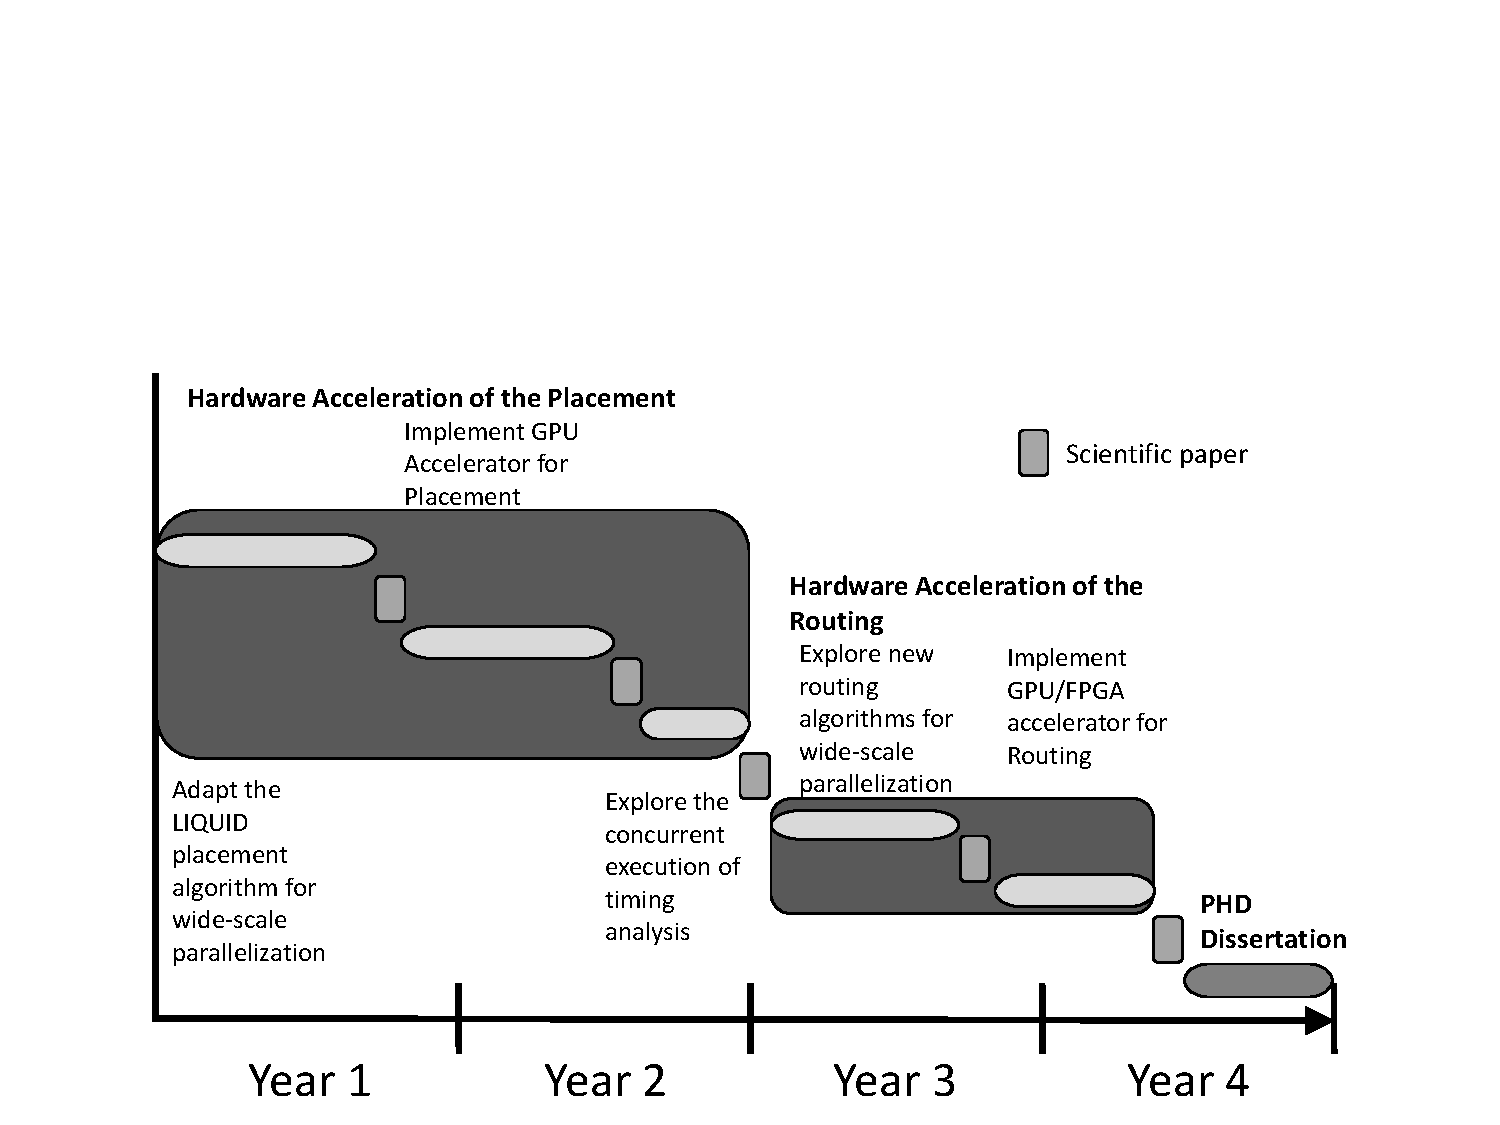
\includegraphics[width = \textwidth,trim = 0mm 0mm 0mm 65mm, clip]{timeschedule.pdf}
\caption{Proposed timetable for the PhD research.}
\label{timeschedule}
\end{figure}




\newpage
%\nocite{*}
\bibliographystyle{phdsymp}
\bibliography{proposal} % commented if *.bbl file included, as
%\bibliography{../../../bib/hes} % commented if *.bbl file included, as
%%%%%see below
%%DIrk_bis: in je referenties hoofdletters escapen door ze tussen {} te zetten, zoals voor {FPGA}'s.

%%%%%%%%%%%%%%%%% BIBLIOGRAPHY IN THE LaTeX file !!!!! %%%%%%%%%%%%%%%%%%%%%%%%
%% This is nothing else than the phdsymp_sample2e.bbl file that you would%%
%% obtain with BibTeX: you do not need to send around the *.bbl file
%%
%%---------------------------------------------------------------------------%%
%
%\begin{thebibliography}{1}
%\bibitem{LaTeX}
%Leslie Lamport,
%\newblock {\em A Document Preparation System: \LaTeX, User's Guide and
%  Reference Manual},
%\newblock Addison Wesley Publishing Company, 1986.
%\bibitem{LaTeXD}
%Helmut Kopka,
%\newblock {\em \LaTeX, eine Einf\"uhrung},
%\newblock Addison-Wesley, 1989.
%\bibitem{TeX}
%D.K. Knuth,
%\newblock {\em The {\rm T\kern-.1667em\lower.7ex\hbox{E}\kern-.125emX}book},
%\newblock Addison-Wesley, 1989.
%\bibitem{METAFONT}
%D.E. Knuth,
%\newblock {\em The {\rm METAFONT}book},
%\newblock Addison Wesley Publishing Company, 1986.
%\end{thebibliography}
%
%%---------------------------------------------------------------------------%%

\end{document}

%%%%%%%%%%%%%%%%%%%%%  End of phdsymp_sample2e.tex  %%%%%%%%%%%%%%%%%%%%%%%%%%%

